


% =================== ARTICLE DEFINITION ===================
\documentclass[a4paper,10pt,english]{article}
%\documentclass[a4paper,twocolumn,10pt]{article}
\setlength{\oddsidemargin}{-.5in}
\setlength{\topmargin}{-.7in}
\setlength{\textheight}{10in} 
\setlength{\textwidth}{7.3in}
\setlength{\parskip}{1em}

%\renewcommand{\thesection}{\Alph{section}.}

% ======================== PACKAGES ========================
\usepackage{graphicx}
\usepackage{amsmath}
\usepackage{cite}
\usepackage{multirow}
\usepackage[utf8]{inputenc}
\usepackage[T1]{fontenc}
\usepackage{lmodern}
\usepackage{blindtext}
\usepackage{enumitem}
\usepackage{url}
\usepackage[table]{xcolor}
\usepackage{multicol}
\usepackage{multirow}

\usepackage{blindtext}

\usepackage{babel}
\usepackage[font=small,labelfont=bf]{caption}
%\usepackage[table,xcdraw]{xcolor}
%\usepackage{dblfloatfix}

\usepackage[ruled,vlined]{algorithm2e}

%\titleformat*{\section}{\small\bfseries}

% ======================= BODY TEXT ========================




\title{Numerical Hand Gesture Classifier}
\author{Jose Millan\\
    \url{jampmil@gmail.com}\\
    Data Mining \& Knowledge Management Masters Program\\
    Università degli Studi del Piemonte Orientale 'Amedeo Avogadro'\\
    Alessandria, Italy}
\date{}



\begin{document}


    \maketitle
    
    \begin{abstract}
        Lorem ipsum dolor sit amet, consectetur adipiscing elit. Duis tempus lacus eget congue tincidunt. Morbi a velit justo. Maecenas consectetur eleifend gravida. Vivamus hendrerit ante vel est dictum vehicula. Quisque venenatis rutrum massa, at consectetur mauris posuere id. Integer fermentum, nulla ac mollis convallis, tellus nunc molestie nunc, eget vulputate mi odio eget nulla. Nulla facilisi. Phasellus tempus diam ligula, non tempus elit tristique ac. Donec volutpat neque a arcu pellentesque facilisis. Fusce a tempor eros. Integer imperdiet turpis vel lacus porta, vitae convallis dui luctus. In lobortis, ex id malesuada fringilla, augue metus mollis ipsum, sed auctor nisi turpis nec arcu. Nulla diam felis, congue a odio vitae, sodales fermentum turpis. Nunc vel hendrerit metus, ultricies ullamcorper ligula. 
    \end{abstract}
    

     \section{Introduction}\label{sec:intro}
     
        Hand gesture recognition implies the use of image processing along with visual data mining to correctly identify specific gestures that are being shown. The current work presents a simple classifier that using a SVM model, is able to identify between five different gestures (numbers from 1 to 5) when they are shown towards a camera.

     \section{Acronym List}
     
        The following acronyms are used through the current work and are necessary to understand its contents.
         
        \begin{itemize}[topsep=0pt,itemsep=0ex,partopsep=1ex,parsep=1ex]
             \item SVM: Support Vector Machine
             \item RGB: Red, Green, Blue
             \item HSV: Hue, Saturation, and Value
             \item OpenCV: Open Source Computer Vision Library
             \item TODO MORE!
         \end{itemize}
     
    \section{Theoretical Assumptions}
    
        \subsection{Thresholding}
        TODO!!!
        
        \subsection{Hue, Saturation, and Value - HSV}
        
        TODO!!!
        
        \subsection{Support Vector Machine - SVM}
        
        Support Vector Machine (SVM) \cite{SVM:Cortes1995} is a supervised machine learning algorithm. This algorithm that can be used for either classification or regression, nevertheless they are more commonly used in classification problems.
        
        SVMs are based on the idea of finding a hyperplane that best divides a dataset into two classes. In the case of a two features problem, as seen in Figure \ref{fig:svm_simple}, a hyperplane as a line that linearly separates and classifies a set of data. The more features the problem has the dimension of the hyperplane increases, due to this its name \cite{SVM:Wiki}.
    
        \begin{figure}[h!]
            \centering
            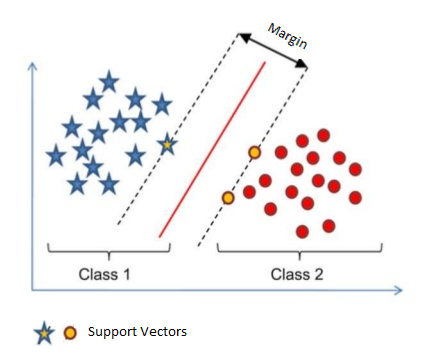
\includegraphics[width=300pt]{images/svm_simple}
            \caption{Simple Visualization of SVM} \label{fig:svm_simple}
        \end{figure}
    
        The further from the hyperplane the  data points lie, the more confident in their correct classification. Considering this the objective of the SVM algorithm is to choose a hyperplane with the greatest possible margin between the hyperplane and any point within the training set, giving a greater chance of new data being classified correctly.
        
        SVM is usually used for text classification tasks such as category assignment, detecting spam and sentiment analysis. It is also commonly used for image recognition challenges, performing particularly well in aspect-based recognition and color-based classification. SVM also plays a vital role in many areas of handwritten digit recognition, such as postal automation services \cite{SVM:Simple}.
        
        \subsection{Cross-Validatino}
        
        TODO!!!
    
    \section{Algorithm Description}\label{sec:algorithms}
    
         The developed solution is divided in four different main tasks, each one necessary for the Hand Gesture Classifier. Below there is a description of each task and its the pseudo-code.
         
         
        \subsection{Preprocess Images}
        
        The first task that is necessary for the Hand Recognition Classifier is to be able to preprocess any image so afterwards its suitable for the model that is being used. For this, an ideal scenario was set, where each hand gesture is shown to the camera against a dark color background.
        
        With this conditions, the image is converted to HSV and then a threshold over its HSV values is applied to the image in order to get a black and white image with the contour of the gesture, where finally a blur effect is applied to soften and improve the contours. With this processed image it is ensured that the model will produce better results compared with an unprocessed image.
    
        \begin{figure}[h!]
            \centering
            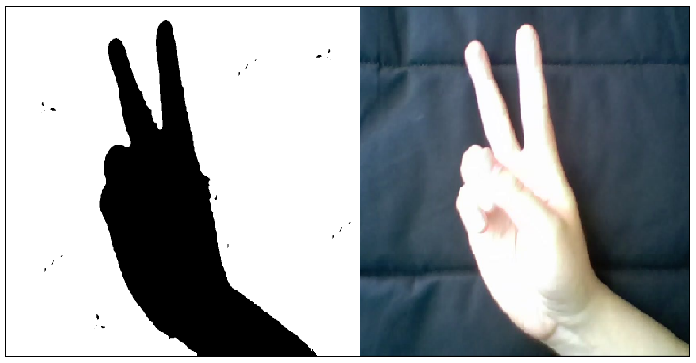
\includegraphics[width=300pt]{images/processing}
            \caption{Final Preprocessing of the a Hand Gesture Image} \label{fig:processing}
        \end{figure}
    
        
        Figure \ref{fig:processing} shows the processed image with its correspondent original image, where the contour of the hand is clear for the model to use the processed image. Algorithm \ref{alg:process_image} shows the steps to process the images and to get the result shown, which in the implementation refers to the function \texttt{Mat processImage(Mat img, int* hsvConfig)}.
        
        \IncMargin{1em}
        \begin{algorithm}[H]
            \KwData{original image, hsv configuration}
            \KwResult{processed image}
            \BlankLine
            \Begin{
                convert image to hsv\;
                threshold original image using the configuration\;
                apply blur\;
                resize image to 640x480\;
            }
            \caption{Process an Image} \label{alg:process_image}
        \end{algorithm}
        
        \subsection{Create Datasets and Train/Test SVM Model}
        
        The next task of the Hand Gesture Classifier is to be able to train a SVM model based on a given dataset of hand gesture images, with their respective class, as it can seen in Algorithm \ref{alg:svm_model}. For this, the program will loop through the folders in the \texttt{images} folder importing and preprocessing the images (using each folder name as the class of the images it contains).
        
        With the images processed then the algorithm divides them in the training and testing sets (with a ratio of \textasciitilde{}30\%), the first one of those is used to create and train an SVM model (using a linear kernel), storing the model in a file (\texttt{HandNumbersClassifier\_01.dat}) and then its performance is tested using the testing set. Finally the algorithm prints the results of the process.
        
        This task is implemented in the function \texttt{void trainSVM()} which itself calls the function \texttt{void createData( Mat\& trainData, Mat\& trainClasses, Mat\&testData, Mat\& testClasses, Ptr<TrainData>\& trainingInData)}.
        
        \begin{algorithm}[H]
            \KwResult{Trained and Tested SVM Model }
            \BlankLine
            \Begin{
                read images folder\;
                process images\;
                divide images in training and testing set\;
                create and train SVM model with training set\;
                write SVN model in file\;
                test model with testing set\;
                print test results\;
            }
            \caption{Create Datasets and Train/Test SVM Model Algorithm} \label{alg:svm_model}
        \end{algorithm}
        
        \subsection{Configure Camera}
        
        The objective of the configure camera task is to find and store the correct configuration of the HSV values for preprocessing the images afterwards. For this two windows are displayed to the user, one with the current video taken from the camera, and another, with sliders for configuring the HSV values, that shows the frames of the video processed with the current HSV values. The user is able to move the sliders to find the right configuration, and when it has been found, pressing any key will finish this task, by storing the HSV values in a configuration file (\texttt{hsv.config}).
        
        Algorithm \ref{alg:configure_camera} shows the pseudo-code of this task which was implemented in the function \texttt{void configureCamera()} of the developed solution.
        
        \begin{algorithm}[H]
            \KwResult{HSV Configuration}
            \BlankLine
            \Begin{
                read stored hsv configuration\;
                configure window with hsv sliders\;
                activate camera\;
                \While{no key is pressed}{
                    process frames of camera with current hsv configuration\;
                    show original camera frames\;
                    show processed camera frames\;
                }
                close windows showed to user\;
                write current hsv configuration\;
            }
            \caption{Configure Camera Algorithm} \label{alg:configure_camera}
        \end{algorithm}
        
        \subsection{Read From Camera and Classify Gestures}
         
         The final task of this work consists in allowing the user perform the hand gestures in front of the camera, where the program will show the user the prediction of which gesture is being presented, while typing the value of the gesture on the console. In order to allow the user change between signs and avoid possible miss interpretations, after a sign has been recognized the program will not attempt to recognize any hand gesture for the next three seconds.
         
         For this the first step is to load the previously created SVN model, along with the stored HSV configuration. Then the camera is started and then the program shows the user three windows: one for the current camera capture, another one with the camera frames processed and finally one that shows the user which gesture is being shown to the camera. Every time the program recognizes a gesture, its value is typed in the console so the user can use it later. Finally the program stops when the user presses any key.
         
         This task was implemented in the function \texttt{void readCameraAndPredict()} and the pseudo-code for this can be seen in Algorithm \ref{alg:read_camera_predict}.
         
         \begin{algorithm}[H]
             \KwResult{predictions of the users gestures}
             \BlankLine
             \Begin{
                 load SVM model\;
                 read stored hsv configuration\;
                 activate camera\;
                 \While{no key is pressed}{
                    process frames of camera with current hsv configuration\;
                    show original camera frames\;
                    show processed camera frames\;
                    predict processed camera frame with SVM model\;
                    \eIf{hand gesture recognized}{
                        show recognized number image to the user\;
                        print recognized number in console\;
                        sleep hand gesture recognition for 3 seconds\;
                    }{
                        show no prediction image to the user\;
                    }
                }
                close windows showed to user\;
            }
            \caption{Read from Camera and Predict Algorithm} \label{alg:read_camera_predict}
        \end{algorithm}
    
    \section{Implementation}
         The program written for this work was developed in \texttt{C++}, using the computer vision and machine learning software library OpenCV \cite{OpenCV} version 3.1. All images captured for this program were taken using a standard webcam of a laptop (USB2.0 HD UVC WebCam) .
         
         As mentioned in Section \ref{sec:intro}, the current work includes five specific hand gestures of the first five numbers, along with the empty background. A sample of this gestures can be seen in Figure \ref{fig:hand_gestures} and would be the only gestures the program can recognize. Additionally, in Figure REF!!!, the final user interface for the Configure Camera task (left) and the Read From Camera and Classify Gestures task (right) can be appreciated.
         
         \begin{figure}[h!]
             \centering
             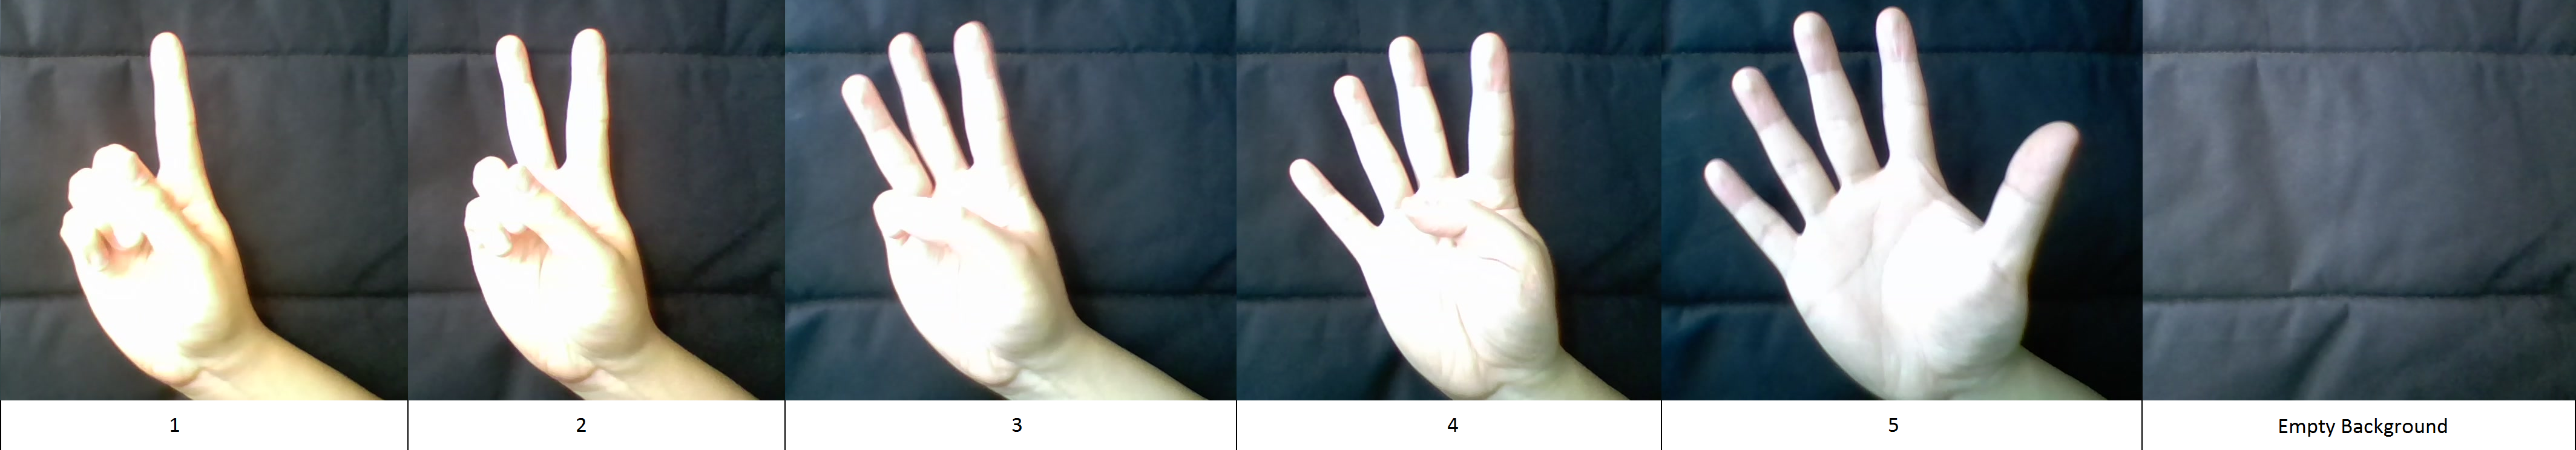
\includegraphics[width=500pt]{images/hand_gestures}
             \caption{Hand Gestures of Numbers from 1 ot 5} \label{fig:hand_gestures}
        \end{figure}
         
         The dataset of these gestures is composed of 926 images (around 150 images per gesture), which were frames taken from videos performing the gesture, by three individuals. These images are stored in the \texttt{images} folder in the root of the program.
         
         
    \section{Tests description}\label{sec:tests}
        
        In order to find the best solution for the Hand Gesture Classifier, two different tasks of the process had to be refined: the preprocessing of the images and tuning the SVM model's parameters.
        
        \begin{enumerate}
            \item Preprocessing Methods:\\
            The first type of tests consist in preprocessing the images before they are passed over the SVM model. The different approaches are described below and a visual sample of them can be appreciated in Figure \ref{fig:test_preprocessing}.
            \begin{enumerate}
                \item No change: This is the default setting for the different tests. It simply consists in no performing any kind of preprocessing to the images.
                \item Gray Scale: Consists in converting the image into its gray scale representation. For this the default values of OpenCV where used, where $gray\_value = 0.30xR + 0.59xG + 0.11xB$
                \item Reduce Color Space: Three different images to test where produced by this method where the representations of each RGB channel was used.
                \item Thresholding: A simple threshold was applied to the image, optimizing its HSV values as explained in Section \ref{sec:algorithms}. For this the image was transformed from RGB to HSV and then the function \texttt{inRange} of the OpenCV library was used.
                \item Thresholding + Blur: A last approach was implemented where the threshold process was performed to the image as described before, and afterwards a noise reduction effect was added in order to reduce the empty spaces within the image. For this a median blur was used using the OpenCV function \texttt{medianBlur} with \texttt{blurSize = 5}.
            \end{enumerate}

            \item SVM Model Tunning:\\
                For the SVM model implemented only a liner kernel was tested (due to satisfactory final results). The challenge then was finding the correct values for the parameters $C$ (error penalty) and $\gamma$ (the linear kernel parameter). In here different values for the parameters were used, restricting the search so $ 0 < C, \gamma <= 10 $ with intervals of 0.5. It is important to understand that for finding the correct values of these parameters, the images used were not processed at all before passing them to the SVM model.
        \end{enumerate}
        
        \begin{figure}[h!]
            \centering
            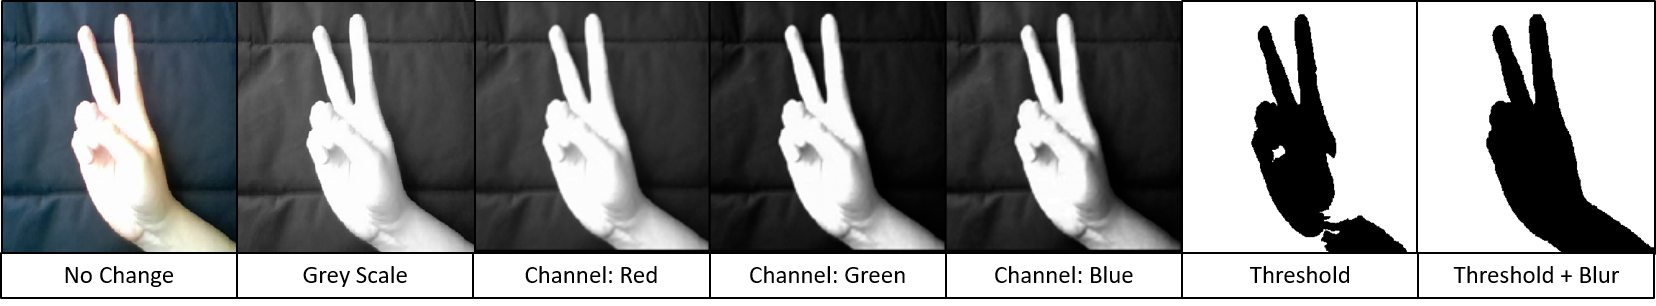
\includegraphics[width=500pt]{images/test_preprocessing}
            \caption{Final Preprocessing of the a Hand Gesture Image} \label{fig:test_preprocessing}
        \end{figure}
                
        In order to perform the tests described before, the dataset was divided into a training and a testing sets, with a radio of around 30\% for the testing set. Finally, when the best combination for the two tasks was found, a 3-fold cross-validation was performed over the results of the trained SVM model, in order to discard any kind of over-fitting in the final model. The results for this process can be seen in Section \ref{sec:results}.
    
    \section{Results}\label{sec:results}
    
    The results of the tests described in Section \ref{sec:tests} are used to find the best process for the Hand Gesture Classifier. Table \ref{tab:preprocessing} shows the results for the different preprocessing methods, whereas Tables \ref{tab:results_gamma} and \ref{tab:results_c} show the results of the SVM model tunning process, which can be graphically appreciated in Figure REF!!.

    \begin{table}[h!]
        \centering
        \caption{Preprocessing Methods Test Results}
        \label{tab:preprocessing}
        \begin{tabular}{|l|c|}
            \hline
            \multicolumn{1}{|c|}{\textbf{Preprocessing Method}} & \textbf{Accuracy on Test} \\ \hline
            No change                                           & 94.245                    \\ \hline
            Grey Scale                                          & 94.964                    \\ \hline
            Reduce color space: Red                             & 94.964                    \\ \hline
            Reduce color space: Green                           & 94.604                    \\ \hline
            Reduce color space: Blue                            & 95.324                    \\ \hline
            Threshold                                           & 96.043                    \\ \hline
            Threshold + Blur                                    & \cellcolor{green!25}96.403                    \\ \hline
        \end{tabular}
    \end{table}
    
    

    
    
    \begin{minipage}{\textwidth}
        \begin{minipage}[b]{0.49\textwidth}
            \centering
            \begin{tabular}{|l|c|}
                \hline
                \multicolumn{1}{|c|}{\textbf{$\gamma$}} & \textbf{Accuracy on Test with} \\ \hline
                0.5                              & 92.446\%                       \\ \hline
                1                                & 92.806\%                       \\ \hline
                1.5                              & 92.806\%                       \\ \hline
                2                                & 93.165\%                       \\ \hline
                2.5                              & 93.885\%                       \\ \hline
                3                                & 94.245\%                       \\ \hline
                3.5                              & 93.885\%                       \\ \hline
                4                                & 94.604\%                       \\ \hline
                4.5                              & 94.245\%                       \\ \hline
                5                                & 94.604\%                       \\ \hline
                5.5                              & \cellcolor{green!25} 94.964\%                       \\ \hline
                6                                & 94.604\%                       \\ \hline
                6.5                              & 94.245\%                       \\ \hline
                7                                & 94.245\%                       \\ \hline
                7.5                              & 93.885\%                       \\ \hline
                8                                & 94.245\%                       \\ \hline
                8.5                              & 93.885\%                       \\ \hline
                9                                & 93.525\%                       \\ \hline
                9.5                              & 92.806\%                       \\ \hline
                10                               & 92.446\%                       \\ \hline
            \end{tabular}
            \captionof{table}{$\gamma$ value vs. Accuracy on Test with C = 0.5}\label{tab:results_gamma}
        \end{minipage}
        \hfill
        \begin{minipage}[b]{0.49\textwidth}
            \centering
                \begin{tabular}{|l|c|}
                    \hline
                    \multicolumn{1}{|c|}{\textbf{$C$}} & \textbf{Accuracy on Test with $\gamma$ = 0.5} \\ \hline
                    0.5                              & 94.604\%                               \\ \hline
                    1                                & 95.324\%                               \\ \hline
                    1.5                              & 94.964\%                               \\ \hline
                    2                                & 95.324\%                               \\ \hline
                    2.5                              & \cellcolor{green!25} 95.683\%                               \\ \hline
                    3                                & 95.324\%                               \\ \hline
                    3.5                              & 94.964\%                               \\ \hline
                    4                                & 94.604\%                               \\ \hline
                    4.5                              & 93.885\%                               \\ \hline
                    5                                & 94.245\%                               \\ \hline
                    5.5                              & 93.165\%                               \\ \hline
                    6                                & 93.525\%                               \\ \hline
                    6.5                              & 92.806\%                               \\ \hline
                    7                                & 92.446\%                               \\ \hline
                    7.5                              & 91.727\%                               \\ \hline
                    8                                & 91.007\%                               \\ \hline
                    8.5                              & 91.367\%                               \\ \hline
                    9                                & 90.647\%                               \\ \hline
                    9.5                              & 90.288\%                               \\ \hline
                    10                               & 90.288\%                               \\ \hline
                \end{tabular}
            \captionof{table}{$C$ value vs. Accuracy on Test with $\gamma$ = 0.5}\label{tab:results_c}
        \end{minipage}
    \end{minipage}
    
    \begin{figure}[h!]
        \centering
        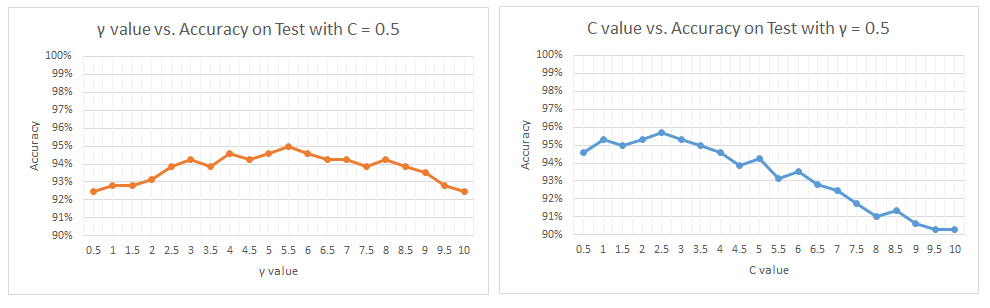
\includegraphics[width=500pt]{images/results_svm_parameters}
        \caption{SVM Parameters Tunning Results} \label{fig:results_svm_parameters}
    \end{figure}
    
    
    With this results the best configuration was defined as using the thresholding + blur method for preprocessing and the parameters $\gamma = 0.55$ and $C = 2.5$ for the SVM model.  As mentioned in Section \ref{sec:tests}, a 3-fold cross-validation was performed over this final process, whose results can be seen in Table \ref{table:cross_val}.
    
    \begin{table*}[h!]
        \centering
        \caption{3-Fold Cross Validation for the SVM Model}
        \label{table:cross_val}
        \begin{tabular}{ | c | c | c | c |  }
            \hline
            Configuration & Accuracy in Training Set & Accuracy in Testing Set & Average Accuracy \\
            \hline
            \multirow{3}{*}{\vtop{\hbox{\strut thresholding + blur}\hbox{\strut $\gamma = 0.55$}\hbox{\strut $C = 2.5$}}} & 99.845 & 98.201 & \cellcolor{green!25}\\
            \cline{2-3}
            & 100 & 97.942 & \cellcolor{green!25}\\
            \cline{2-3}
            & 99.746 & 98.178 & \cellcolor{green!25}\multirow{-3}{*}{98.107}\\
            \hline
            
        \end{tabular}
    \end{table*}
    
    
    \section{Conclusions and Future Work}
    
    Lorem ipsum dolor sit amet, consectetur adipiscing elit. Duis tempus lacus eget congue tincidunt. Morbi a velit justo. Maecenas consectetur eleifend gravida. Vivamus hendrerit ante vel est dictum vehicula. Quisque venenatis rutrum massa, at consectetur mauris posuere id.
    

     
   \bibliographystyle{plain}
   \vspace{5ex}\bibliography{report} 
    
\end{document}   

 